\documentclass[10pt]{article}
\usepackage{lingmacros}
\usepackage{tree-dvips}
\usepackage{setspace}
\usepackage{amsmath}
\usepackage{biblatex}
\usepackage{amsmath}
\usepackage{pgfplots}
\pgfplotsset{compat=1.18}
\addbibresource{references.bib}

\begin{document}

\onehalfspacing% This sets the line spacing to 1.5

\section*{Galaxy simulation}
\section*{Gravitationskraft mit und ohne Plummer Softening}

Die Gravitationskraft ohne Softening ist durch das Newtonsche Gravitationsgesetz gegeben:

\begin{equation}
F = G \frac{m_1 m_2}{r^2}
\end{equation}

Mit Plummer-Softening wird die Kraft modifiziert, um Singularitäten bei sehr kleinen Abständen zu vermeiden. Die modifizierte Kraft lautet:

\begin{equation}
F_{\text{Plummer}} = G \frac{m_1 m_2}{(r^2 + \epsilon(r)^2)^{3/2}}
\end{equation}

wobei \(\epsilon(r) = \frac{\epsilon_0}{1 + r^2}\) eine Funktion des Abstands \(r\) ist, die bei kleinen \(r\) einen konstanten Wert annimmt und bei großen \(r\) gegen null geht.

Hier ist $\epsilon_0$ der Softening-Parameter.

\begin{center}
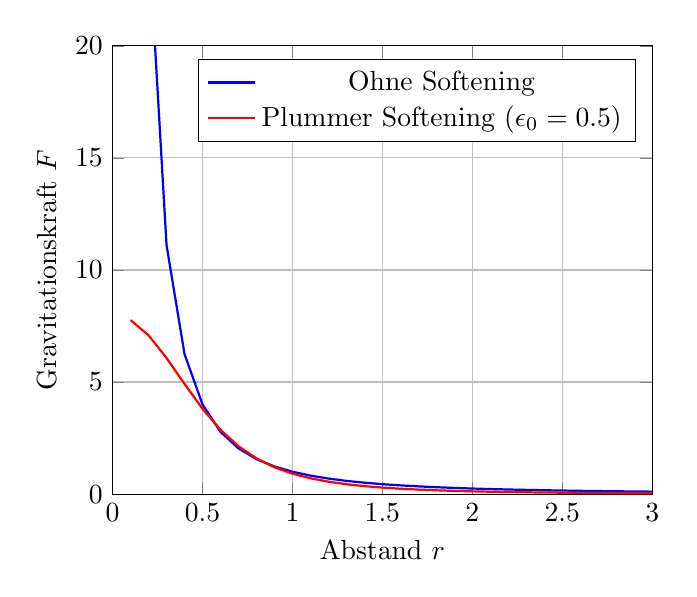
\begin{tikzpicture}
\begin{axis}[
    xlabel={Abstand $r$},
    ylabel={Gravitationskraft $F$},
    ymin=0, ymax=20, xmin=0, xmax=3,
    legend pos=north east,
    grid=major,
    domain=0.1:10,
    samples=100
]
\addplot[
    color=blue,
    thick
]
{1/x^2};
\addlegendentry{Ohne Softening}

\addplot[
    color=red,
    thick
]
{1/(x^2 + (0.5/(1 + x^2))^2)^(3/2)};
\addlegendentry{Plummer Softening ($\epsilon_0 = 0.5$)}

\end{axis}
\end{tikzpicture}
\end{center}

\subsection*{Introduction}

The goal of this project is to simulate the evolution of a galaxy over time. The simulation will be based on the N-body problem, which describes the motion of a group of celestial objects interacting with each other through gravitational forces. The simulation will model the galaxy as a collection of stars, each of which will be represented as a point mass. The stars will interact with each other through gravitational forces, causing them to move and change their positions over time. The simulation will be implemented using a numerical integration method, such as the Runge-Kutta method, to solve the equations of motion for the stars \cite{binney2008galactic}.

\subsection*{Methodology}

The simulation will be implemented in Python using the NumPy library for numerical computations \cite{harris2020array}. The galaxy will be modeled as a two-dimensional system, with each star represented as a point mass with a position and velocity. The stars will interact with each other through gravitational forces, which will be calculated using Newton's law of gravitation \cite{newton1687principia}. The simulation will be run for a fixed period of time, during which the positions and velocities of the stars will be updated at regular intervals. The simulation will be visualized using a plotting library, such as Matplotlib, to show the evolution of the galaxy over time \cite{hunter2007matplotlib}.

\subsection*{Derivation of the Expansion of the Universe}

Starting with the Friedmann equations, which describe the evolution of the scale factor of the universe over time. The Friedmann equations are given by:

\begin{equation}
\left(\frac{\dot{a}}{a}\right)^2 = \frac{8\pi G}{3} \rho - \frac{k}{a^2}
\end{equation}

\begin{equation}
\frac{\ddot{a}}{a} = -\frac{4\pi G}{3} (\rho + 3p)
\end{equation}

where $a(t)$ is the scale factor of the universe, $\rho(t)$ is the energy density, $p(t)$ is the pressure, and $k$ is the curvature of the universe \cite{friedmann1922}. The first Friedmann equation describes the expansion rate of the universe, while the second Friedmann equation describes the acceleration of the expansion.

The expansion of the universe can be described by the Hubble parameter, which is defined as:

\begin{equation}
H(t) = \frac{\dot{a}}{a}
\end{equation}

The Hubble parameter is a measure of the rate of expansion of the universe, and it is related to the energy density and pressure of the universe through the Friedmann equations \cite{hubble1929}. The Hubble parameter can be used to calculate the age of the universe, the distance to distant galaxies, and the rate of expansion of the universe.

Assuming a flat universe with $k = 0$, the Friedmann equations can be simplified to:

\begin{equation}
H^2 = \frac{8\pi G}{3} \rho
\end{equation}

\begin{equation}
\frac{\ddot{a}}{a} = -\frac{4\pi G}{3} (\rho + 3p)
\end{equation}

where H is the Hubble parameter, $\rho$ is the energy density, and p is the pressure of the universe. The expansion of the universe can be described by the scale factor $a(t)$, which represents the size of the universe at time t. The scale factor can be used to calculate the age of the universe, the distance to distant galaxies, and the rate of expansion of the universe \cite{peebles1993principles}.

\subsection*{Mathematical Theory}

The motion of the stars in the galaxy will be governed by Newton's law of gravitation, which states that the gravitational force between two objects is proportional to the product of their masses and inversely proportional to the square of the distance between them \cite{newton1687principia}. The equation of motion for a star in the galaxy can be written as:

\begin{equation}
m_i \frac{d^2\mathbf{r}_i}{dt^2} = \sum_{j \neq i} G \frac{m_i m_j}{|\mathbf{r}_i - \mathbf{r}_j|^3} (\mathbf{r}_j - \mathbf{r}_i)
\end{equation}

where $m_i$ and $m_j$ are the masses of the stars, $\mathbf{r}_i$ and $\mathbf{r}_j$ are their positions, and $G$ is the gravitational constant. The equation of motion can be solved numerically using a numerical integration method, such as the Runge-Kutta method, to update the positions and velocities of the stars at each time step \cite{press1992numerical}.

That leads to the acceleration being calculated as:

\begin{equation}
\mathbf{a}_i(t) = \sum_{j \neq i} G \frac{m_j}{|\mathbf{r}_i(t) - \mathbf{r}_j(t)|^3} (\mathbf{r}_j(t) - \mathbf{r}_i(t))
\end{equation}

where $m_j$ is the mass of the star $j$ and $\mathbf{r}_j$ is its position.

So the position of the star at time $t + \Delta t$ can be calculated as:

\begin{equation}
\mathbf{r}_i(t + \Delta t) = \mathbf{r}_i(t) + \mathbf{v}_i(t) \Delta t + \frac{1}{2} \mathbf{a}_i(t) \Delta t^2
\end{equation}

where $\mathbf{v}_i$ is the velocity of the star and $\mathbf{a}_i$ is the acceleration, which can be calculated from the gravitational forces acting on the star. The velocities of the stars can be updated using a similar equation \cite{binney2008galactic}.

% diagramm wich shows the acceleration, velocity and position of a star


\subsection*{Results}

The simulation will produce a visual representation of the galaxy at different points in time, showing how the stars move and interact with each other over time. The simulation will allow us to study the dynamics of the galaxy and observe how it evolves over time. By varying the initial conditions of the simulation, such as the number of stars and their initial positions and velocities, we can explore how different factors affect the evolution of the galaxy. The simulation will provide valuable insights into the formation and evolution of galaxies and help us better understand the dynamics of these complex systems \cite{toomre1972}.

\subsection*{Conclusion}

In conclusion, this project aims to simulate the evolution of a galaxy over time using the N-body problem. The simulation will model the galaxy as a collection of stars interacting with each other through gravitational forces. The simulation will be implemented in Python using the NumPy library and visualized using a plotting library. The results of the simulation will provide valuable insights into the dynamics of galaxies and help us better understand the formation and evolution of these complex systems \cite{springel2005cosmological}.

\printbibliography

\end{document}
 